\documentclass[11pt,a4paper]{article}

\usepackage[a4paper,left=3.5cm, right=2.5cm, top=3.5cm, bottom=3.5cm]{geometry}
\usepackage[dutch]{babel}
\usepackage{amsmath}
\usepackage{tikz}
\usepackage{graphicx}
\usepackage{pdfpages}

\setlength\parindent{0pt}                   % Fix stupid indentation on new line
\setlength\parskip{\medskipamount}

\title{Activiteitenrapport 2}
\author{Olivier Van den Eede}
\date{\today}

\begin{document}
    \maketitle
    
    \section{Reeds uitgevoerde activiteiten}
        \subsection{Algemeen}
            Op basis van de opmerkingen van de jury over de tussentijdse presentatie en verslag is er beslist om een duidelijker doel te stellen.
            De opgestelde planning was te ambitieus, en niet haalbaar in de resterende tijd. Om deze reden heb ik een duidelijker doel proberen te stellen dat haalbaar zou moeten zijn.

            De focus zal vanaf nu liggen op object-detectie en het linken van deze objecten aan kenmerken op een semantische kaart.
            Het deel over segmentatie zal verder niet meer onderzocht worden omdat het annoteren en trainen van een segmentatienetwerk te veel tijd in beslag zou nemen.

            Meer details kunnen gevonden worden in de bijgevoegde planning.

        \subsection{Annotatie beeldmateriaal}
            Om een object-detector te maken gebaseerd op een CNN moet al het nieuw verkregen beeldmateriaal geannoteerd worden door bounding-boxes te teken
            rondom kenmerkende objecten en deze ook een bijhorend label te geven. Dit is een tijdrovend proces en heeft een hoeveelheid tijd in beslag genomen.
            Een opsomming van alle annotaties in de training en de validatie dataset is terug te vinden in tabel~\ref{tab:annotaties}.

            \begin{table}[h]
                \caption{Annotaties in training en validatie set}\label{tab:annotaties}
                \begin{tabular}{l | l | l | l | l | l | l}
                    & Aantal frames & Rookmelder & Deurklink & Pictogram & TL-lamp & Totaal \\ \hline
                    Trainings set & 899 & 1016 & 147 & 340 & 5260 & 6763 \\
                    Validatie set & 711 & 1130 & 180 & 408 & 992 & 2710 \\
                \end{tabular}
            \end{table}


        \subsection{Training CNN}
            Als object-detector heb ik gekozen om gebruik te maken van YOLO-V2 in de originele Darknet implementatie.
            De training van het netwerk is begonnen op basis van de pretrained YOLO-V2-voc weights. 
            Het netwerk wordt momenteel getraind om 4 object classen te detecteren zoals in tabel~\ref{tab:annotaties} beschreven. 
            Het trainen is nog volop aan de gang, zoals te zien in figuur~\ref{fig:training_loss} is de gemiddelde loss van de training reeds een stuk gezakt, maar nog niet goed genoeg.
        

            \begin{figure}[!htb]
                \centering
                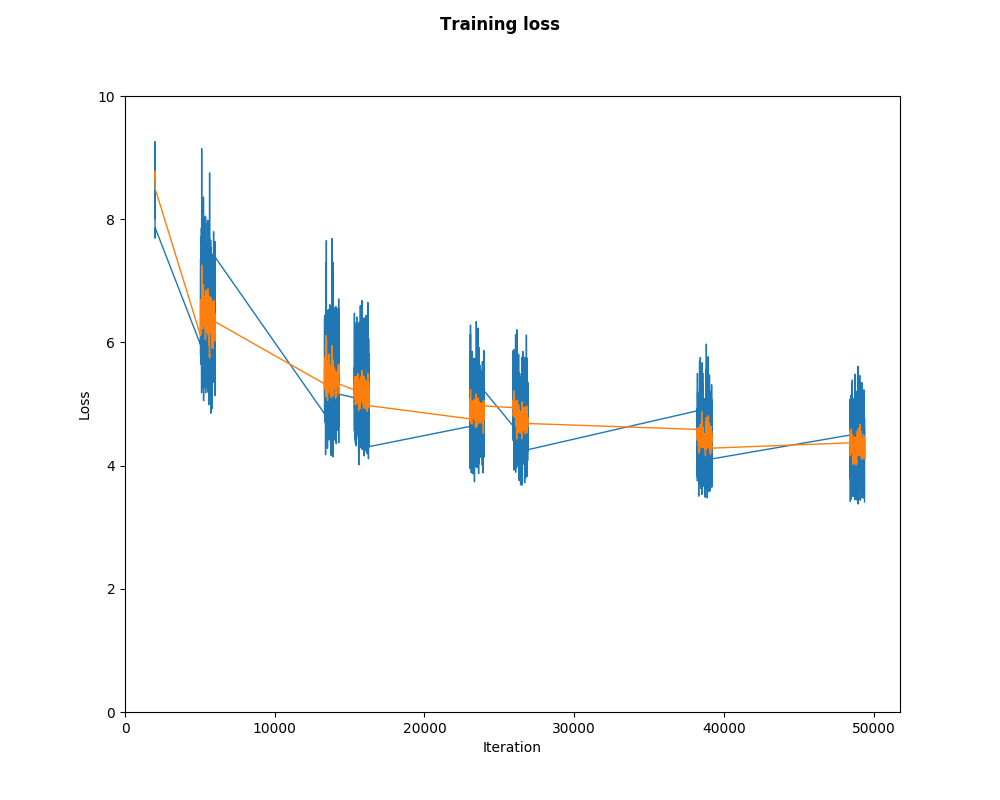
\includegraphics[width=\linewidth]{training_loss_12_2.png}
                \caption{Plot van de gemiddelde training loss}
                \label{fig:training_loss}
            \end{figure}

    \section{Uit te voeren activiteiten}
        \begin{itemize}
            \item Verder trainen netwerk
            \item Valideren object-detector en accuracy bepalen
            \item Gedetecteerde objecten linken met kenmerken uit semantische kaart
            \item Thesis schrijven
        \end{itemize}

    % \bibliographystyle{plain}
    % \bibliography{literatuur.bib}
    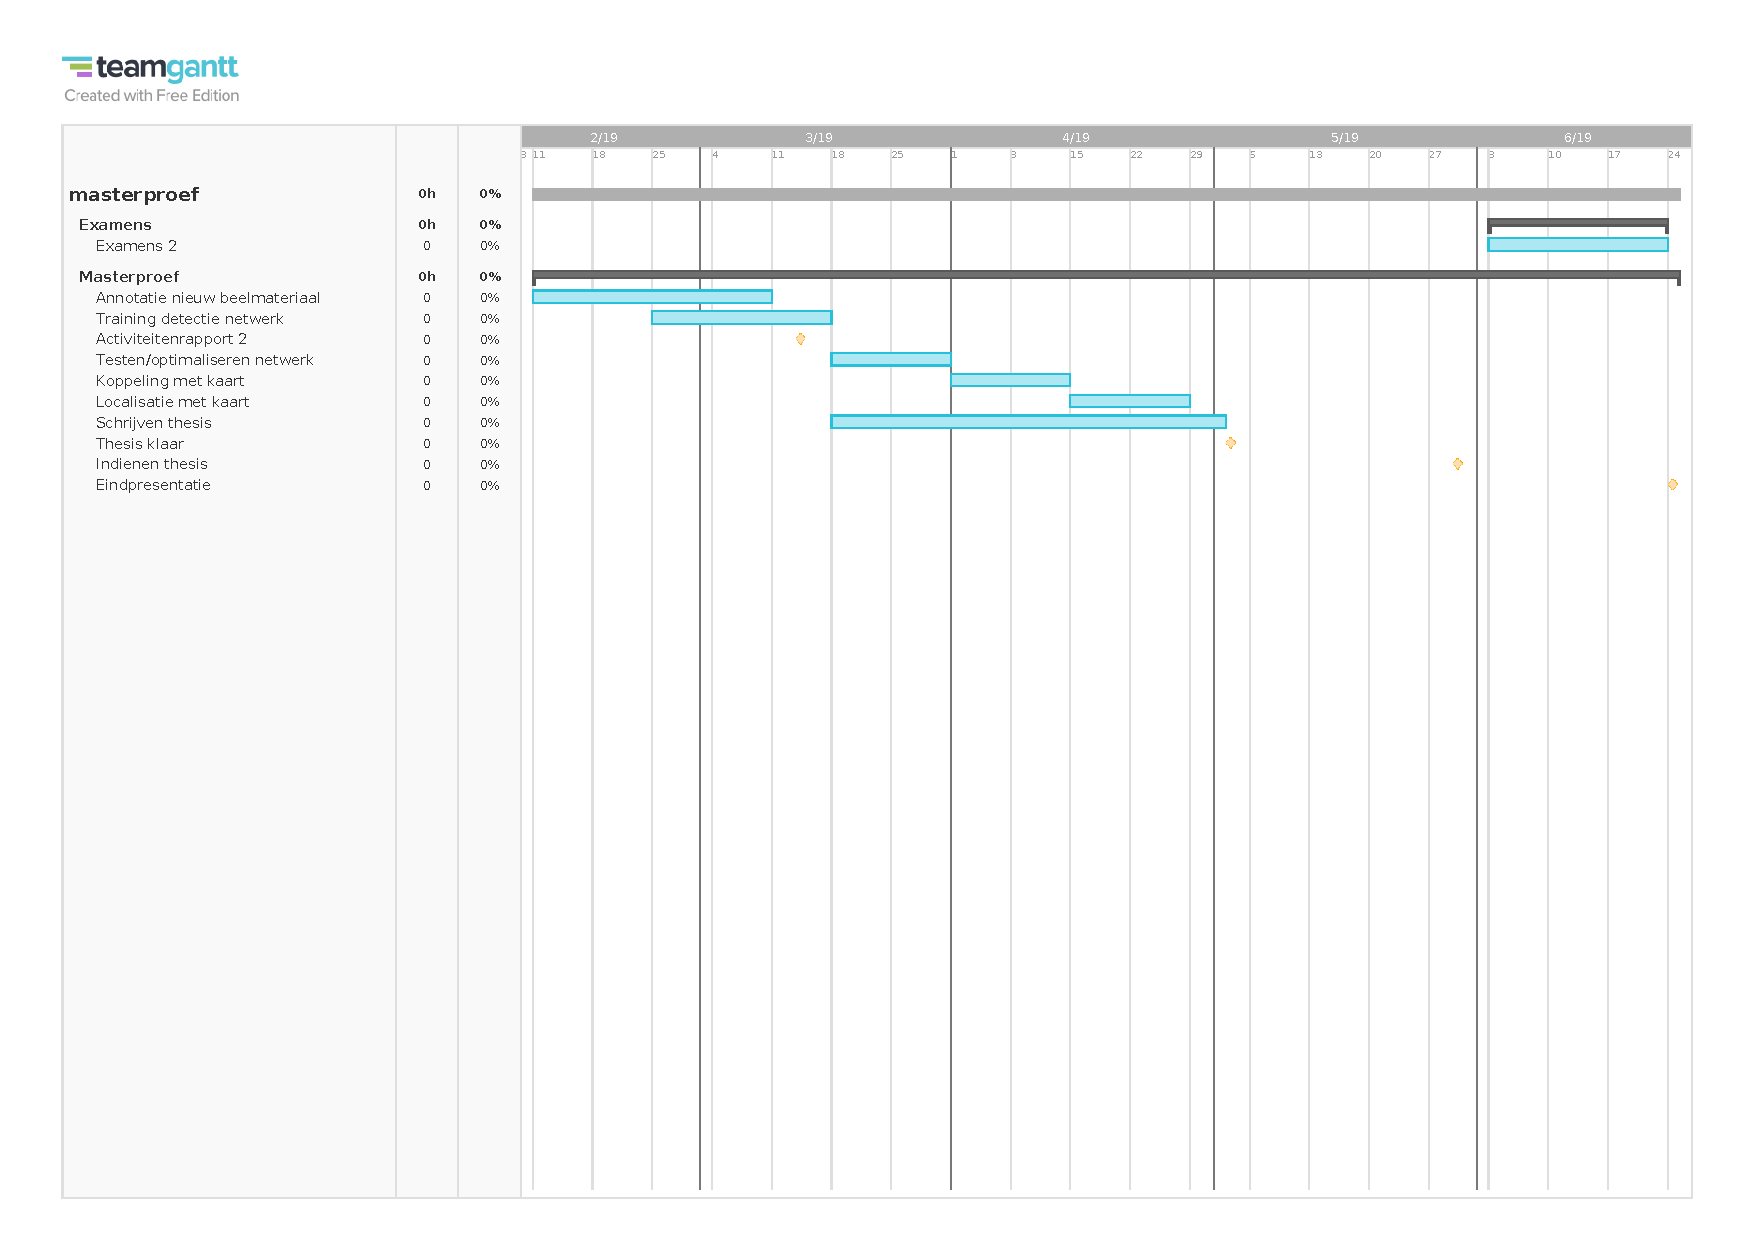
\includepdf[landscape=true]{planning.pdf}

\end{document}